% THIS DOCUMENT IS TAILORED TO REQUIREMENTS FOR SCIENTIFIC COMPUTING.  IT SHOULDN'T
% BE USED FOR NON-SCIENTIFIC COMPUTING PROJECTS
\documentclass[12pt]{article}

\usepackage{amsmath, mathtools}
\usepackage{amsfonts}
\usepackage{amssymb}
\usepackage{graphicx}
\usepackage{colortbl}
\usepackage{xr}
\usepackage{hyperref}
\usepackage{longtable}
\usepackage{xfrac}
\usepackage{tabularx}
\usepackage{float}
\usepackage{siunitx}
\usepackage{booktabs}
\usepackage{caption}
\usepackage{pdflscape}
\usepackage{afterpage}

\usepackage[round]{natbib}

%\usepackage{refcheck}

\hypersetup{
    bookmarks=true,         % show bookmarks bar?
      colorlinks=true,       % false: boxed links; true: colored links
    linkcolor=red,          % color of internal links (change box color with linkbordercolor)
    citecolor=green,        % color of links to bibliography
    filecolor=magenta,      % color of file links
    urlcolor=cyan           % color of external links
}



% For easy change of table widths
\newcommand{\colZwidth}{1.0\textwidth}
\newcommand{\colAwidth}{0.13\textwidth}
\newcommand{\colBwidth}{0.82\textwidth}
\newcommand{\colCwidth}{0.1\textwidth}
\newcommand{\colDwidth}{0.05\textwidth}
\newcommand{\colEwidth}{0.8\textwidth}
\newcommand{\colFwidth}{0.17\textwidth}
\newcommand{\colGwidth}{0.5\textwidth}
\newcommand{\colHwidth}{0.28\textwidth}

% Used so that cross-references have a meaningful prefix
\newcounter{defnum} %Definition Number
\newcommand{\dthedefnum}{GD\thedefnum}
\newcommand{\dref}[1]{GD\ref{#1}}
\newcounter{datadefnum} %Datadefinition Number
\newcommand{\ddthedatadefnum}{DD\thedatadefnum}
\newcommand{\ddref}[1]{DD\ref{#1}}
\newcounter{theorynum} %Theory Number
\newcommand{\tthetheorynum}{T\thetheorynum}
\newcommand{\tref}[1]{T\ref{#1}}
\newcounter{tablenum} %Table Number
\newcommand{\tbthetablenum}{T\thetablenum}
\newcommand{\tbref}[1]{TB\ref{#1}}
\newcounter{assumpnum} %Assumption Number
\newcommand{\atheassumpnum}{P\theassumpnum}
\newcommand{\aref}[1]{A\ref{#1}}
\newcounter{goalnum} %Goal Number
\newcommand{\gthegoalnum}{P\thegoalnum}
\newcommand{\gsref}[1]{GS\ref{#1}}
\newcounter{instnum} %Instance Number
\newcommand{\itheinstnum}{IM\theinstnum}
\newcommand{\iref}[1]{IM\ref{#1}}
\newcounter{reqnum} %Requirement Number
\newcommand{\rthereqnum}{P\thereqnum}
\newcommand{\rref}[1]{R\ref{#1}}
\newcounter{nfrnum} %NFR Number
\newcommand{\rthenfrnum}{NFR\thenfrnum}
\newcommand{\nfrref}[1]{NFR\ref{#1}}
\newcounter{lcnum} %Likely change number
\newcommand{\lthelcnum}{LC\thelcnum}
\newcommand{\lcref}[1]{LC\ref{#1}}

\usepackage{fullpage}

\newcommand{\deftheory}[9][Not Applicable]
{
\newpage
\noindent \rule{\textwidth}{0.5mm}

\paragraph{RefName: } \textbf{#2} \phantomsection 
\label{#2}

\paragraph{Label:} #3

\noindent \rule{\textwidth}{0.5mm}

\paragraph{Equation:}

#4

\paragraph{Description:}

#5

\paragraph{Notes:}

#6

\paragraph{Source:}

#7

\paragraph{Ref.\ By:}

#8

\paragraph{Preconditions for \hyperref[#2]{#2}:}
\label{#2_precond}

#9

\paragraph{Derivation for \hyperref[#2]{#2}:}
\label{#2_deriv}

#1

\noindent \rule{\textwidth}{0.5mm}

}

\begin{document}

\title{Software Requirements Specification for Truss Tool: 
A Tool for Truss Analysis} 
\author{Maryam Valian}
\date{\today}
	
\maketitle

~\newpage

\pagenumbering{roman}

\tableofcontents

~\newpage

\section*{Revision History}

\begin{tabularx}{\textwidth}{p{3cm}p{2cm}X}
\toprule {\bf Date} & {\bf Version} & {\bf Notes}\\
\midrule
 2023-01-30 & 1.0 & Initial version of the SRS\\
Date 2 & 1.1 & Notes\\
\bottomrule
\end{tabularx}

~\newpage

\section{Reference Material}

This section records information for easy reference.

\subsection{Table of Units}

Throughout this document, SI (Syst\`{e}me International d'Unit\'{e}s) is employed
as the unit system.  In addition to the basic units, several derived units are
used as described below.  For each unit, the symbol is given followed by a
unit description and the SI name.
~\newline

\renewcommand{\arraystretch}{1.2}
%\begin{table}[ht]
  \noindent \begin{tabular}{l l l} 
    \toprule		
    \textbf{symbol} & \textbf{unit} & \textbf{SI}\\
    \midrule 
    \si{\metre} & length & metre\\
    \si{\newton} & force & newton\\
    \si{\deg} & angle & degree\\
        \bottomrule
  \end{tabular}
  %	\caption{Provide a caption}
%\end{table}

\subsection{Table of Symbols}

The table that follows summarizes the symbols used in this document along with
their units.  The choice of symbols was made to be consistent with the structural statics literature and with existing documentation for the truss analysis problem. The symbols are listed in alphabetical order.

\renewcommand{\arraystretch}{1.2}
%\noindent \begin{tabularx}{1.0\textwidth}{l l X}
\noindent \begin{longtable*}{l l p{12cm}} \toprule
\textbf{symbol} & \textbf{unit} & \textbf{description}\\
\midrule 
$F_\text{i}$ & \si {\newton} & External force of joint i \\
$M_\text{i}$ & \si{\newton}\si{\metre} & Moment component of joint i \\
$\theta$ & \si{\deg} & Angle between two members  \\
$F_\text{xi}$ & \si{\newton} & Force component in the x direction of joint i \\
$F_\text{yi}$ & \si{\newton} & Force component in the y direction of joint i \\
$S_\text{p}$ & - & Pin support \\
$S_\text{r}$ & - & Roller support \\

\bottomrule
\end{longtable*}


\subsection{Abbreviations and Acronyms}

\renewcommand{\arraystretch}{1.2}
\begin{tabular}{l l} 
  \toprule		
  \textbf{symbol} & \textbf{description}\\
  \midrule 
  A & Assumption\\
  DD & Data Definition\\
  GD & General Definition\\
  GS & Goal Statement\\
  IM & Instance Model\\
  LC & Likely Change\\
  PS & Physical System Description\\
  R & Requirement\\
  SRS & Software Requirements Specification\\
 
  T & Theoretical Model\\
  \bottomrule
\end{tabular}\\



\subsection{Mathematical Notation}
In this document, we do not use any specific mathematical notation.

\newpage

\pagenumbering{arabic}

%{When the documentation is done, it should be possible to trace back to the source of every piece of information.  Some information will come from  external sources, like terminology.  Other information will be derived, like  General Definitions.
%An SRS document should have the following qualities: unambiguous,  consistent, complete, validatable, abstract and traceable.{The overall goal of the SRS is that someone that meets the Characteristics  of the Intended Reader (Section~\ref{sec_IntendedReader}) can learn,  understand and verify the captured domain knowledge.  They should not have to   trust the authors of the SRS on any statements.  They should be able to  independently verify/derive every statement made.}


\section{Introduction}
{A truss is a structure that consists of members organized into connected triangles to enable the distribution of loads and forces. Trusses are most commonly used for wide spans like bridges, and roofs. Truss Analysis shows whether the external forces are well-distributed among the members or not. \\
The following section provides an overview of the software requirements specification (SRS) for the truss tool. In this section, first, we explain the purpose of the document. Then we explain the scope of the requirements, the characteristics of the intended reader and the organization of the document.
}
%The introduction section is written to introduce the problem.  It starts  general and focuses on the problem domain. The general advice is to start with a paragraph or two that describes the problem, followed by a ``roadmap'' paragraph.  A roadmap orients the reader by telling them what sub-sections to expect in the Introduction section.}

\subsection{Purpose of Document}
{The primary purpose of this document is to outline the software requirements of the truss analysis tool. To provide a good understanding of the system, different aspects of the system such as  goals, assumptions, theoretical models, and definitions will be explained.  The following SRS document will remain abstract exploring what is being solved rather than how it will be solved.\\
The following document will describe the system context and constraints, the specific problem definition and solution characteristics, requirements and likely and unlikely changes for the 
development of the tool.}
%\plt{This section summarizes the purpose of the SRS document.  It does not focus  on the problem itself.  The problem is described in the ``Problem  Description'' section (Section~\ref{Sec_pd}).  The purpose is for the document  in the context of the project itself, not in the context of this course.  Although the ``purpose'' of the document is to get a grade, you should not  mention this.  Instead, ``fake it'' as if this is a real project.  The purpose  section will be similar between projects.  The purpose of the document is the  purpose of the SRS, including communication, planning for the design stage,  etc.}

\subsection{Scope of Requirements} 
{The scope of the requirements includes the analysis of the two-dimensional trusses where all members and nodes lie within a two-dimensional plane. for more details, you can also see the assumptions section  (Section~\ref{sec_assumpt}). }
%\plt{Modelling the real world requires simplification.  The full complexity of   the actual physics, chemistry, biology is too much for existing models, and  for existing computational solution techniques.  Rather than say what is in   the scope, it is usually easier to say what is not.  You can think of it as  the scope is initially everything, and then it is constrained to create the  actual scope.  For instance, the problem can be restricted to 2 dimensions, or  it can ignore the effect of temperature (or pressure) on the material   properties, etc.}  

%\plt{The scope section is related to the assumptions section  (Section~\ref{sec_assumpt}).  However, the scope and the assumptions are not   at the same level of abstraction.  The scope is at a high level.  The focus is on the ``big picture'' assumptions.  The assumptions section lists, and  describes, all of the assumptions.}

\subsection{Characteristics of Intended Reader} \label{sec_IntendedReader}
Reviewers of this documentation should have a basic understanding of structure statics and high school physics and Mathematics. The users of the Truss Tool must have a higher level of expertise, as explained in Section: User Characteristics (Section~\ref{SecUserCharacteristics}). 

\subsection{Organization of Document}
The organization of the document follows the template for an SRS for scientific computing software proposed by \citet{SmithandLai2005}. The template will present the system's goals, theories, definitions, and assumptions. Readers interested in top-down reading can begin by reading the system's goal statements (Section~\ref{Sec_gs}). Subsequently, the theoretical models will elaborate on the goal statements. Lastly, readers can finish with a more  understanding of the system by reading instance models of the system.

\section{General System Description}

This section provides general information about the system.  It identifies the interfaces between the system and its environment, describes the user characteristics and lists the system constraints.  %\plt{This text can likely be borrowed verbatim.}

%\plt{The purpose of this section is to provide general information about the  system so the specific requirements in the next section will be easier to  understand. The general system description section is designed to be changeable independent of changes to the functional requirements documented in  the specific system description. The general system description provides a   context for a family of related models.  The general description can stay the  same, while specific details are changed between family members.}

\subsection{System Context}
Figure~\ref{Fig_SystemContext} shows the system context. The circles 
represent a user that interacts with the software. The rectangle represents the software system for the truss tool. The arrows display the input data from the user and the output data that is useful for the user.
%\plt{Your system context will include a figure that shows the abstract view of   the software.  Often in a scientific context, the program can be viewed   abstractly following the design pattern of Inputs $\rightarrow$ Calculations   $\rightarrow$ Outputs.  The system context will therefore often follow this  pattern.  The user provides inputs, the system does the calculations and then  provides the outputs to the user.  The figure should not show all of the  inputs, just an abstract view of the main categories of inputs (like material  properties, geometry, etc.).  Likewise, the outputs should be presented from  an abstract point of view.  In some cases, the diagram will show other external  entities, besides the user.  For instance, when the software product is a  library, the user will be another software program, not an actual end user.  If there are system constraints that the software must work with external  libraries, these libraries can also be shown on the System Context diagram.  They should only be named with a specific library name if this is required by the system constraint.}

\begin{figure}[h!]
\begin{center}
 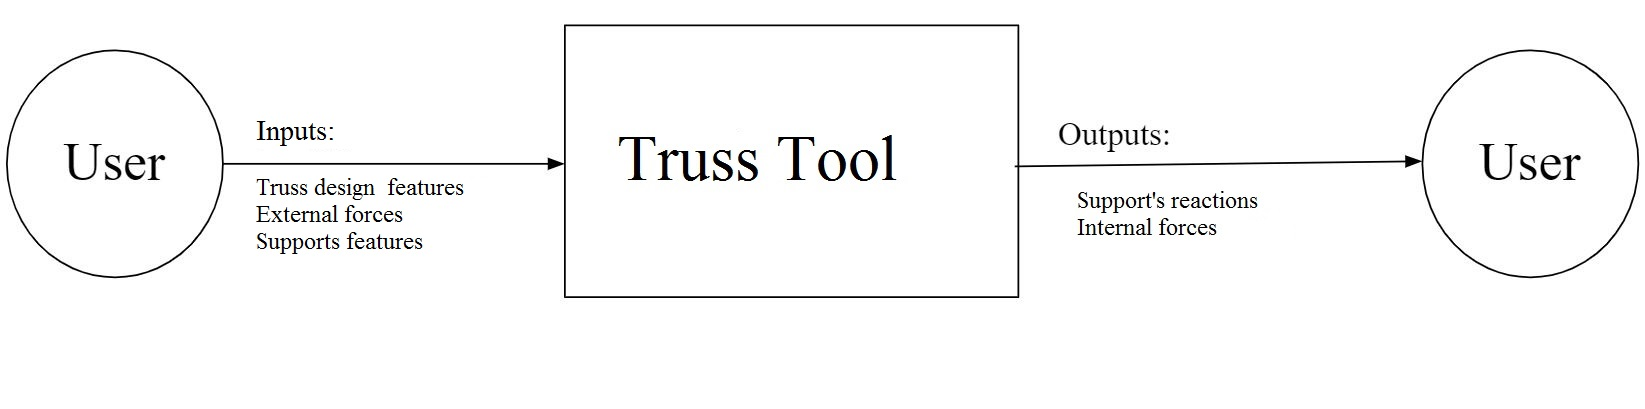
\includegraphics[width=0.8\textwidth]{systemcontext.jpg}
\caption{System Context}
\label{Fig_SystemContext} 
\end{center}
\end{figure}

The interaction between the product and the user is through a user interface. The responsibilities of the user and the system are as follows:
\begin{itemize}
\item User Responsibilities:
\begin{itemize}
\item Provide truss design features, supports and external forces. 
\item Ensure the input data describes a correct truss.

\end{itemize}
\item Truss Tool Responsibilities:
\begin{itemize}
\item Detect data type mismatch, such as a string of characters instead of a  floating point number.
\item Calculate external forces and support's reaction.
\end{itemize}
\end{itemize}


\subsection{User Characteristics} \label{SecUserCharacteristics}

The end user of Truss Tool should be an architecture/civil/mechanic engineer or should have an understanding of undergraduate Level 1 structural analysis.

\subsection{System Constraints}

There is no constraint on the development of the Truss Tool.


\section{Specific System Description}

This section first presents the problem description, which gives a high-level view of the problem to be solved.  This is followed by the solution characteristics specification, which presents the assumptions, theories, definitions and finally the instance models.


\subsection{Problem Description} \label{Sec_pd}

Truss Tool is intended to solve a given truss with given external forces. By solving a truss, we mean that we are interested to calculate all internal forces among the members and the reactions of the supports. As a result, Truss Tool will help engineers to make a decision on whether the design of the given truss is proper or not.


\subsubsection{Terminology and  Definitions}


This subsection provides a list of terms that are used in the subsequent
sections and their meaning, with the purpose of reducing ambiguity and making it easier to correctly understand the requirements:

\begin{itemize}

\item{ Planar truss:  A planar truss is one where all members and nodes lie within a two-dimensional plane.} 
\item{Joint(nodes): A place where two or more  members of the truss  are connected.}
\item{Force equilibrium: A body is in force equilibrium if the sum of all the forces acting on the body is zero.}
\item{Moment equilibrium: A body is in moment equilibrium if the sum of all the moments of all the forces acting on the body is zero.}
\item{Moment: The turning effect of a force is called the moment. The moment is the result of the force multiplied by the perpendicular distance from the line of action of the force to the pivot or point where the object will turn.}
\item{Compression: When a member force points toward the joint it is attached to, the member is in compression}
\item{Tension: When a member force points away from the joint it is attached to, the member is in tension.}
\item{Pinned support: A kind of structural support that can have both a horizontal reaction and a vertical reaction. }
\item{Roller support: A kind of structural support that can have only a vertical reaction. }
\item{Zero force members: Members which do not have any force in them.}
\end{itemize}

\subsubsection{Physical System Description} \label{sec_phySystDescrip}

%\plt{The purpose of this section is to clearly and unambiguously state the physical system that is to be modelled. Effective problem-solving requires a logical and organized approach. The statements on the physical system to be studied should cover enough information to solve the problem. The physical   description involves element identification, where elements are defined as   independent and separable items of the physical system. Some example elements include acceleration due to gravity, the mass of an object, and the size and   shape of an object. Each element should be identified and labelled, with its interesting properties specified clearly. The physical description can also include interactions of the elements, such as the following: i) the interactions between the elements and their physical environment; ii) the interactions between elements; and, iii) the initial or boundary conditions.}

The physical system of the Truss Tool, as shown in Figure~\ref{fig_physys},
includes the following elements:

\begin{itemize}

\item{PS1: The joints ($j_\text{1}$,$j_\text{2}$,..,$j_\text{n}$).}
\item{PS2: The members ($m_\text{1}$,$m_\text{2}$,..,$m_\text{k}$).}
\item{PS3: The supports ($S_\text{1}$,$S_\text{2}$).}

\end{itemize}

%\plt{A figure here makes sense for most SRS documents}

 \begin{figure}[h!]
\begin{center}
 %\rotatebox{-90}
 
  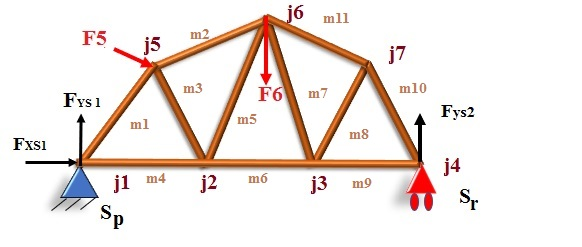
\includegraphics[width=0.7\textwidth]{physic_system.jpg}
 
 \caption{The physical system of Truss Tool}
 \label{fig_physys}
 \end{center}
 \end{figure}

\subsubsection{Goal Statements} \label{Sec_gs}

%\plt{The goal statements refine the ``Problem Description''   (Section~\ref{Sec_pd}).  A goal is a functional objective the system under   consideration should achieve. Goals provide criteria for sufficient  completeness of a requirements specification and for requirements  pertinence. Goals will be refined in Section “Instanced Models”  (Section~\ref{sec_instance}). Large and complex goals should be decomposed  into smaller sub-goals.  The goals are written abstractly, with a minimal  amount of technical language.  They should be understandable by non-domain  experts.}

\noindent Given the truss features and external forces, the goal statements are:

\begin{itemize}
\item{GS\refstepcounter{goalnum}\thegoalnum \label{G_react}: Calculate the reactions of the supports.}
\item{GS\refstepcounter{goalnum}\thegoalnum \label{G_force}: Calculate the internal forces for each member.}
\end{itemize}

\subsection{Solution Characteristics Specification}

%\plt{This section specifies the information in the solution domain of the system   to be developed. This section is intended to express what is required in   such a way that analysts and stakeholders get a clear picture, and the latter will accept it. The purpose of this section is to reduce the problem  into one expressed in mathematical terms. Mathematical expertise is used to   extract the essentials from the underlying physical description of the problem, and to collect and substantiate all physical data pertinent to the problem.}

%This section presents the solution characteristics by successively refining   models.  It starts with the abstract/general Theoretical Models (TMs) and refines them to the concrete/specific Instance Models (IMs). 
%If necessary there are intermediate refinements to General Definitions (GDs).  All of these refinements can potentially use Assumptions (A) and Data Definitions (DD). TMs are refined to create new models, that are called GMs or IMs. DDs are not refined; they are just used. GDs and IMs are derived, or refined, from other   models. DDs are not derived; they are just given. 
%--------->TMs are also just given, but  they are refined, not used.  If a potential DD includes a derivation, then that means it is refining other models, which would make it a GD or an IM.}

%\plt{The above makes a distinction between ``refined'' and ``used.'' A model is refined to another model if it is changed by the refinement. When we change a general 3D equation to a 2D equation, we are making a refinement, by applying the assumption that the third dimension does not matter. If we use a definition, like the definition of density, we aren't refining, or changing that definition, we are just using it.}

%\plt{The same information can be a TM in one problem and a DD in another.  It is about how the information is used.  In one problem the definition of acceleration can be a TM, in another, it would be a DD.}

%\plt{There is repetition between the information given in the different chunks  (TM, GDs etc) with other information in the document.  For instance, the  meaning of the symbols, the units etc are repeated.  This is so that the chunks can stand on their own when being read by a reviewer/user.  It also facilitates reuse of the models in a different context.}

%\noindent \plt{The relationships between the parts of the document are show in  the following figure.  In this diagram ``may ref'' has the same role as `uses'' above.  The figure adds ``Likely Changes,'' which are able to reference (use) Assumptions.}

%\begin{figure}[H]
%  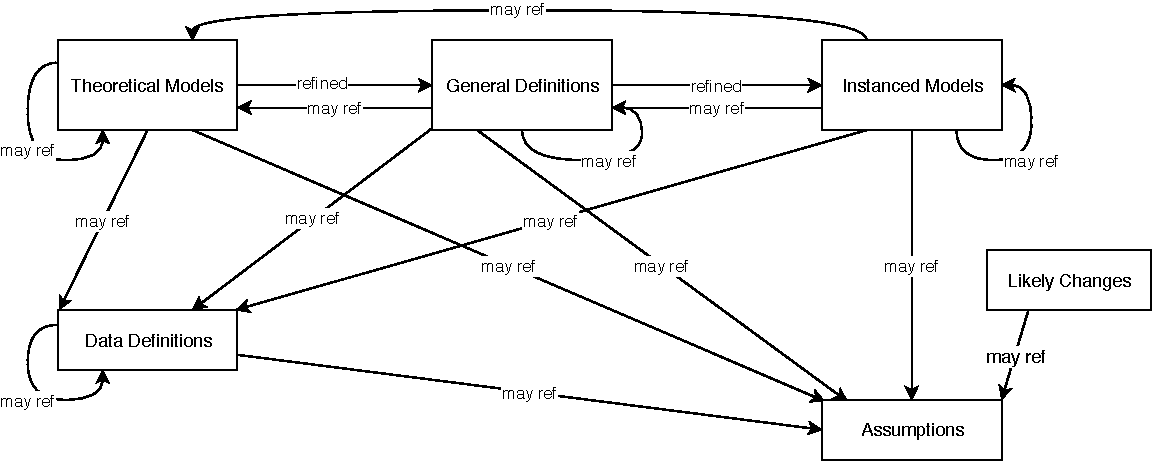
\includegraphics[scale=0.9]{RelationsBetweenTM_GD_IM_DD_A.pdf}
%\end{figure}

The instance models that govern Truss Tool are presented in
Subsection~\ref{sec_instance}.  The information to understand the meaning of the instance models and their derivation is also presented so that the instance models can be verified.

\subsubsection{Assumptions} \label{sec_assumpt}

%\plt{The assumptions are a refinement of the scope.  The scope is general, where the assumptions are specific.  All assumptions should be listed, even those that domain experts know so well that they are rarely (if ever) written down.}
%\plt{The document should not take for granted that the reader knows which assumptions have been made. In the case of unusual assumptions, it is  recommended that the documentation either include, or point to, an explanation  and justification for the assumption.}

This section simplifies the original problem and helps in developing the
theoretical model by filling in the missing information for the physical
system. The numbers given in the square brackets refer to the theoretical model
[T], the general definition [GD], data definition [DD], instance model [IM], or
likely change [LC], in which the respective assumption is used.

\begin{itemize}

\item{A\refstepcounter{assumpnum}\theassumpnum \label{planar}: All members and nodes lie within a two-dimensional plane.}

\item{A\refstepcounter{assumpnum}\theassumpnum \label{connection}: Members are inter-connected only at their ends.}
\item{A\refstepcounter{assumpnum}\theassumpnum \label{as_straight}: Members must be straight.}
\item{A\refstepcounter{assumpnum}\theassumpnum \label{frictionless}: All joints are smooth and frictionless hinges.}
\item{A\refstepcounter{assumpnum}\theassumpnum \label{Force_at_joints}: All forces must only be applied at joints}
\item{A\refstepcounter{assumpnum}\theassumpnum \label{reaction_at_joints}: All reactions must only be applied at joints}
\item{A\refstepcounter{assumpnum}\theassumpnum \label{self_w}: Self-weight of the member will be neglected}
\item{A\refstepcounter{assumpnum}\theassumpnum \label{axial_fmem}: Members are subjected to axial forces only.}
\item{A\refstepcounter{assumpnum}\theassumpnum \label{maxsupport}: The number of supports at most is two.}


%  \plt{Short description of each assumption.  Each assumption     should have a meaningful label.  Use cross-references to identify the    appropriate traceability to T, GD, DD etc., using commands like dref, ddref etc.  Each assumption should be atomic - that is, there should not be an explicit (or implicit) ``and'' in the text of an assumption.}

\end{itemize}

\subsubsection{Theoretical Models}\label{sec_theoretical}

%\plt{Theoretical models are sets of abstract mathematical equations or axioms for solving the problem described in Section ``Physical System Description''  (Section~\ref{sec_phySystDescrip}). Examples of theoretical models are physical laws, constitutive equations, relevant conversion factors, etc.}

This section focuses on the general equations and laws that Truss Tool is based on. 
%\plt{Modify the examples below for your problem, and add additional models as appropriate.}

~\newline

\noindent
\deftheory
% #2 refname of theory
{T: EQUIL}
% #3 label
{ Equilibrium Equations}
% #4 equation
{
$\sum F = 0$ ,  & $\sum M = 0$\\
 
}
% #5 Description
{  
   
 
  & The equilibrium equation describes the static equilibrium of all  forces of the system and the moment for the system so that $\sum M =0$ and $\sum F=0$.\\
  & $F$ is any force in the system (\si{\newton}). $M$ is a moment that is the turning effect of a force. Moments act about a point in a clockwise or anticlockwise direction(\si{\newton\metre})\\
}
% #6 Notes
{ 
None.
}
% #7 Source
{
  \url{https://en.wikipedia.org/wiki/Mechanical_equilibrium/}
}
% #8 Referenced by
{
  \dref{Trussequil}
}
% #9 Preconditions
{
None
}
% #1 derivation - not applicable by default
{}
%----------------------------------------------------

\newpage
~\newline

\subsubsection{General Definitions}\label{sec_gendef}

This section collects the laws and equations that will be used in building the
instance models.
%--------------------------------------GD1
~\newline

\noindent
\begin{minipage}{\textwidth}
\renewcommand*{\arraystretch}{1.5}
\begin{tabular}{| p{\colAwidth} | p{\colBwidth}|}
\hline
\rowcolor[gray]{0.9}
Number& GD\refstepcounter{defnum}\thedefnum \label{Trussequil}\\
\hline
Label &\bf Equilibrium equations in planar trusses \\
\hline
SI Units& All Forces are measured in \si{\newton}\\
\hline
Equation& $\sum F_{x}=0 $, $\sum F_{y}=0 $   \\
& $F_{x}=F\cos{\theta}$ , $F_{y}=F\sin{\theta}$\\
\hline
Description &
By Decomposition of the force $F$ into $F_{x}, F_{y}$ (\aref{planar}), For any joint point in a planar truss, the equilibrium equations are satisfied horizontally and vertically in the direction of the x-axis and y-axis.

\\
\hline
  Source & \url{https://www.khanacademy.org/math/geometry/hs-geo-analytic-geometry/hs-geo-distance-and-midpoints/a/distance-formula} \\
  \hline
  Ref.\ By & \iref{Supp_react},\iref{i_force}\\
  \hline
\end{tabular}
\end{minipage}\\

\subsubsection{Data Definitions}\label{sec_datadef}

This section collects and defines all the data needed to build the instance models. The dimension of each quantity is also given. 

~\newline

\noindent
\begin{minipage}{\textwidth}
\renewcommand*{\arraystretch}{1.5}
\begin{tabular}{| p{\colAwidth} | p{\colBwidth}|}
\hline
\rowcolor[gray]{0.9}
Number& DD\refstepcounter{datadefnum}\thedatadefnum \label{length_mem}\\
\hline
Label& \bf Length of a straight Line \\
\hline
Symbol &$L$\\
\hline

  SI Units & \si{\metre}\\
  \hline
  Equation&$L = \sqrt{(x_{2}-x_{1})^2+(y_{2}-y_{1})^2}$\\
 \hline
Description & 
   For every two points such as $X_{1}$,$X_{2}$   with coordination $(x_{1},y_{1})$ and $(x_{2},y_{2})$ the length of line between two point is $L$. \\
  \hline
  Sources& \url{https://www.cuemath.com/distance-formula/} \\
  \hline
  Ref.\ By & \iref{Design_truss}\\
  \hline
\end{tabular}
\end{minipage}\\
%------------------------------------DD2
~\newline


\noindent
\begin{minipage}{\textwidth}
\renewcommand*{\arraystretch}{1.5}
\begin{tabular}{| p{\colAwidth} | p{\colBwidth}|}
\hline
\rowcolor[gray]{0.9}
Number& DD\refstepcounter{datadefnum}\thedatadefnum \label{Law_cos}\\
\hline
Label& \bf Finding angle by Law of cosine \\
\hline
Symbol &$\theta$\\
\hline

  SI Units & Degree\\
  \hline
  Equation& $\theta= \arccos(\frac{a^2+b^2+c^2}{2ab}$)\\
 \hline
Description & 
   The Law of Cosine helps us to find any angle for a  given triangle with a known length of sides. Where $\theta$ is the angle between sides a and b. and c is the length of the opposite side. \\
  \hline
  Sources& \url{https://en.wikipedia.org/wiki/Law_of_cosines} \\
  \hline
  Ref.\ By & \iref{Design_truss}\\
  \hline
\end{tabular}
\end{minipage}\\
\subsubsection{Data Types}\label{sec_datatypes}

This section collects and defines all the data types needed to document the models. For Truss Tool, all data types are real numbers or boolean numbers.

\subsubsection{Instance Models} \label{sec_instance}    

This section transforms the problem defined in Section~\ref{Sec_pd} into 
one which is expressed in mathematical terms. It uses concrete symbols defined 
in Section~\ref{sec_datadef} to replace the abstract symbols in the models 
identified in Sections~\ref{sec_theoretical} and~\ref{sec_gendef}.

The goals \gsref{G_react} and \gsref{G_force} are solved by \iref{Design_truss}, \iref{Supp_react}, \iref{i_force}
 
~\newline

%--------------------Instance Model 1

\noindent
\begin{minipage}{\textwidth}
\renewcommand*{\arraystretch}{1.5}
\begin{tabular}{| p{\colAwidth} | p{\colBwidth}|}
  \hline
  \rowcolor[gray]{0.9}
  Number& IM\refstepcounter{instnum}\theinstnum \label{Design_truss}\\
  \hline
  Label& \bf Calculate truss design features \\
  \hline
  Input& $J_{i}=$ Tuples of $(X,Y)$ location of joints \\& $M_{j}=$ Tuples of end-joints for the members \\
 
   \hline
   Output& $L(m_{j})=$ Tuples of the length of all members such that $0 \leq L$ \\
   &$\theta_{p,q}= $ Tuples of all angles between two members $M_{p}$ and $M_{q}$ so that $0<\theta<180$ \\
   \hline
  Description&  For each member, Truss Tool should calculate the length $L(m_{j})$ from \ddref{length_mem}. For each two members $M_{p}$ and $M_{q}$, Truss Tool should calculate $\theta_{p,q}$ from \ddref{Law_cos}.\\
  
 \hline
  Sources& \url{https://engcourses-uofa.ca/books/statics/structural-analysis/analysis-of-trusses/} \\
  \hline
  Ref.\ By & \iref{i_force}\\
  \hline
\end{tabular}
\end{minipage}\\
~\newline

%----------------------Instance Model 2-------------------
\noindent
\begin{minipage}{\textwidth}
\renewcommand*{\arraystretch}{1.5}
\begin{tabular}{| p{\colAwidth} | p{\colBwidth}|}
  \hline
  \rowcolor[gray]{0.9}
  Number& IM\refstepcounter{instnum}\theinstnum \label{Supp_react}\\
  \hline
  Label& \bf Find support's reactions \\
  \hline
  Input&   $S_{k}=$ Tuples of Joint index for support position $J_{i}$, and type of support from the set of $\{"pin", "roller"\}$\\
  & $F_{i}=$ Tuples of a joint index for the position of an external force, and the amount of force (\si{\newton}) \\ 

  \hline
  Output& $R_ix$, $R_iy$ for each support located on joint $i$, such that if support is a roller one, $R_{ix}=0$ \\

  \hline
  Description & By considering the whole truss as a free body, The reaction of the supports should be calculated from GD\ref{Trussequil} \\
 & The input is constrained so that $k \leq 2$ (\aref{maxsupport})\\
   & For inputting the position of an External force or support, the index of a join is needed. (\aref{Force_at_joints},\aref{reaction_at_joints}) \\
 \hline
  Sources& \url{https://engcourses-uofa.ca/books/statics/structural-analysis/analysis-of-trusses/} \\
  \hline
  Ref.\ By & \iref{i_force},\gsref{G_react}\\
  \hline
\end{tabular}
\end{minipage}\\

~\newline

%----------------------------Instance Model 3

\noindent
\begin{minipage}{\textwidth}
\renewcommand*{\arraystretch}{1.5}
\begin{tabular}{| p{\colAwidth} | p{\colBwidth}|}
  \hline
  \rowcolor[gray]{0.9}
  Number& IM\refstepcounter{instnum}\theinstnum \label{i_force}\\
  \hline
  Label& \bf Calculate internal forces for all members  $IF_{m}$\\
  \hline
  Input& $F_{i}=$ External forces.\\
  & $L(m_{j})$ all Members lengths, $\theta_{p,q}$ all angles between members from \iref{Design_truss}\\
  & $R_{i}$ Support reactions from \iref{Supp_react}\\
  \hline
   Output& $IF_{m}$ Internal force for each member $m$ (\si{\newton})\\
  \hline
  Description& By decomposition of each internal force $IF_{i}$ to $IF_{x}$ and $IF_{y}$ (\aref{planar}) and applying equilibrium equations from GD\ref{Trussequil} for each joint, the internal forces will be calculated jointly. For the last joint $j_{n}$, there will be no unknown internal force left. Hence we can use the last equation as the verification test of output correctness.  \\
 
 \hline
  Sources& \url{https://engcourses-uofa.ca/books/statics/structural-analysis/analysis-of-trusses/} \\
  \hline
  Ref.\ By & \gsref{G_force}\\
  \hline
\end{tabular}
\end{minipage}\\
~\newline
%-----------------------------
\subsubsection{Input Data Constraints} \label{sec_DataConstraints}    

Table~\ref{TblInputVar} shows the data constraints on the input-output
variables.  The column for physical constraints gives the physical limitations
on the range of values that the variable can take.  The column for software constraints restricts the range of inputs to reasonable values.  The software constraints will be helpful in the design stage for picking suitable algorithms.  The constraints are conservative, allowing the model user to experiment with unusual situations.  The column of typical values is intended to provide a feel for a common scenario.  The uncertainty column estimates the confidence with which the physical quantities can be
measured.  This information would be part of the input if one were performing an
uncertainty quantification exercise.\\
The specification parameters in Table~\ref{TblInputVar} are listed in
Table~\ref{TblSpecParams}.

\begin{table}[!h]
  \caption{Input Variables} \label{TblInputVar}
  \renewcommand{\arraystretch}{1.2}
\noindent \begin{longtable*}{l l l l c} 
  \toprule
  \textbf{Var} & \textbf{Physical Constraints} & \textbf{Software Constraints} &
                             \textbf{Typical Value} & \textbf{Uncertainty}\\
  \midrule 
  $n$ & $n > 3$ & $n_{\text{min}} \leq n \leq n_{\text{max}}$ & 8  & 5\%
  \\
  \bottomrule
\end{longtable*}
\end{table}

\noindent 
\begin{description}

\item[(*)] The count of Joints in a given truss is an integer number. it must be greater or equal to 3 to be considered a triangle. For small trusses, the number of joints is around 8. The maximum number of joints $n_{max}$ for the run time considerations will be considered 30.
\end{description}

\begin{table}[!h]
\caption{Specification Parameter Values} \label{TblSpecParams}
\renewcommand{\arraystretch}{1.2}
\noindent \begin{longtable*}{l l} 
  \toprule
  \textbf{Var} & \textbf{Value} \\
  \midrule 
  $n_\text{min}$ & 3 \\
  $n_\text{max}$ & 30\\
  \bottomrule
\end{longtable*}
\end{table}

\subsubsection{Properties of a Correct Solution} \label{sec_CorrectSolution}

\noindent
Table~\ref{TblOutputVar} shows the physical constraints on the output. Suppose all joints from index 1 to $n-1$ are solved. Then all $IF_{m}$ are already calculated and the last joint will be considered as a physical constraint on the output.

\begin{table}[!h]
\caption{Output Variables} \label{TblOutputVar}
\renewcommand{\arraystretch}{1.2}
\noindent \begin{longtable*}{l l} 
  \toprule
  \textbf{Var} & \textbf{Physical Constraints} \\
  \midrule 
  $\sum F_{n}=0$ &  (by~\aref{planar},\aref{Force_at_joints})
  \\
  \bottomrule
\end{longtable*}
\end{table}

\section{Requirements}

This section provides the functional requirements and the business tasks that the
software is expected to be complete, and the nonfunctional requirements, the
qualities that the software is expected to exhibit.

\subsection{Functional Requirements}

\noindent \begin{itemize}

\item{R\refstepcounter{reqnum}\thereqnum \label{R_Inputs}: Input the values from Table \ref{TblInputVal}}

\item{R\refstepcounter{reqnum}\thereqnum \label{R_OutputInputs}:Echoing inputs as part of output.} 

\item{R\refstepcounter{reqnum}\thereqnum \label{R_Calculate}: Calculate support reactions from \iref{Supp_react}, and internal forces from \iref{Design_truss}, \iref{Supp_react}, \iref{i_force}}

\item{R\refstepcounter{reqnum}\thereqnum \label{R_VerifyOutput}: Check summation of internal forces is zero in the last joint. \iref{i_force}}
 \end{itemize}
\begin{table}[!h]
	\caption{Required Inputs} \label{TblInputVal}
	\renewcommand{\arraystretch}{1.2}
	\noindent \begin{longtable*}{l l l l c} 
		\toprule
		\textbf{Symbol} & \textbf{Description} & \textbf{Data Type} \\
		\midrule 
		$F$  & External forces on each joint Index  & Array of Integer (\si{\newton}). \\
		$J$  & The location of all joint & Array of Real tuples \\
		$M$  & A pair of joint index for all members &Array of Integer tuples \\
		
		$S_1, S_2$ & pair of Joint Index as Location of supports and type of support   &(Integer, Char) \\
		\bottomrule
		
	\end{longtable*}
\end{table}

\subsection{Nonfunctional Requirements}



\noindent \begin{itemize}

\item[NFR\refstepcounter{nfrnum}\thenfrnum \label{NFR_Accuracy}:]
  \textbf{Accuracy: The accuracy of the computed solutions should meet the level needed for
structural mechanic and have the properties described in Section \ref{sec_CorrectSolution}.}
 
\item[NFR\refstepcounter{nfrnum}\thenfrnum \label{NFR_Usability}:] \textbf{Usability: The properties of the software should be able to tested easily through
verification and validation plan (VnV Plan).}
 

\item[NFR\refstepcounter{nfrnum}\thenfrnum \label{NFR_Maintainability}:]
  \textbf{Maintainability: The effort required to make any of the likely    changes listed for Truss Tool should be less than 30\% of the original    development time.}

\item[NFR\refstepcounter{nfrnum}\thenfrnum \label{NFR_Portability}:]
  \textbf{Portability:  Truss Tool is runnable on different environments, such as Windows, Mac-OS, and Linux.} 

\end{itemize}

\section{Likely Changes}    

\noindent \begin{itemize}

\item[LC\refstepcounter{lcnum}\thelcnum\label{LC_planar}:] The software may be changed to solve both types of trusses: two-dimensional and three-dimensional [\aref{planar}]  
\item[LC\refstepcounter{lcnum}\thelcnum\label{LC_friction}:] The software may be changed to consider friction of the joints [\aref{frictionless} ]

\end{itemize}

\section{Unlikely Changes}    

\noindent \begin{itemize}

\item[UC1\label{UC_connection}:] The truss members are only connected at their joints [\aref{connection}]
\item[UC2\label{UC_straight}:] The truss members are straight [\aref{as_straight}]
\end{itemize}

\section{Traceability Matrices and Graphs}

The purpose of the traceability matrices is to provide easy references on what
has to be additionally modified if a certain component is changed.  Every time a
component is changed, the items in the column of that component that is marked
with an ``X'' may have to be modified as well.  Table~\ref{Table:trace} shows the
dependencies of theoretical models, general definitions, data definitions, and
instance models with each other. Table~\ref{Table:R_trace} shows the
dependencies of instance models, requirements, and data constraints on each
other. Table~\ref{Table:A_trace} shows the dependencies of theoretical models,
general definitions, data definitions, instance models, and likely changes in
the assumptions.

\begin{table}[h!]
\centering
\begin{tabular}{|c|c|c|c|c|c|c|c|}
\hline
	& T1& \dref{Trussequil}& \ddref{length_mem}  
  & \ddref{Law_cos} &\iref{Design_truss}& \iref{Supp_react}& 
	\iref{i_force}  \\
\hline
T1       & & & & & & &\\ \hline
\dref{Trussequil}    &X & & & & & &\\ \hline
\ddref{length_mem}    & & & & & & &\\ \hline
\ddref{Law_cos}       & & & & & & &\\ \hline
\iref{Design_truss} & & &X &X & & &\\ \hline 
\iref{Supp_react} & &X & & & & &\\ \hline 
\iref{i_force} & &X & & &X &X &\\ \hline 
\end{tabular}
\caption{Traceability Matrix Showing the Connections Between  theoretical models, general definitions,
data definitions and Instance Models}
\label{Table:trace}
\end{table}
%----------------
\begin{table}[h!]
\centering
\begin{tabular}{|c|c|c|c|c|}
\hline
	& \iref{Design_truss}& \iref{Supp_react}& 
	\iref{i_force}& Constraint \ref{sec_DataConstraints}  \\
\hline
R1      &X & & &X\\ \hline
R2    &X & &  &X\\ \hline
R3    &X &X &X&\\ \hline
R4       & & & &X\\ \hline
\end{tabular}
\caption{Traceability Matrix Showing the Connections Between Requirements and Instance Models}
\label{Table:R_trace}
\end{table}
%--------------------
\begin{table}[h!]
\centering
\begin{tabular}{|c|c|c|c|c|c|c|c|c|c|c|}
\hline
	& \aref{planar}& \aref{connection}& \aref{as_straight}  &\aref{frictionless} & \aref{Force_at_joints} & \aref{reaction_at_joints} & \aref{self_w} 
 & \aref{axial_fmem} &\aref{maxsupport}\\
\hline
T1      & & & & & & & & & \\ \hline
\dref{Trussequil}      &X & & &X & & & & & \\ \hline
\ddref{length_mem}      & & &X & & & & & & \\ \hline
\ddref{Law_cos}      & &X &X & & & & & & \\ \hline
\iref{Design_truss}      & &X &X & & & & & & \\ \hline
\iref{Supp_react}      &X &X &X &X &X &X & & &X \\ \hline
\iref{i_force}      &X & & &X & & &X &X &X \\ \hline
\end{tabular}
\caption{Traceability Matrix Showing the Connections Between assumptions and other sections}
\label{Table:A_trace}
\end{table}


\section{Development Plan}

This section is optional.  It is used to explain the plan for developing the software.  In particular, this section gives a list of the order in which the requirements will be implemented.


\section{Values of Auxiliary Constants}
\begin{table}[h!]
	\renewcommand{\arraystretch}{1.2}
	\noindent \begin{longtable*}{l l l l c} 
		\toprule
		\textbf{Symbol} & \textbf{Description} & \textbf{Value} & 
		\textbf{Units} \\
		\midrule 
		$F_{\text{max}}$ & the maximum value for external force & 35000 & 
		\si{\newton}\\
		$F_{\text{min}}$ & the minimum value for external force & -35000 & 
		\si{\newton}\\
        $(X, Y)$ & the maximum value for the distance from the center of the coordinate axis & +20 & 
		\si{\metre}\\
        $(X, Y)$ & the minimum value for the distance from the center of the coordinate axis & 0 & 
		\si{\metre}\\
  	
		$\theta_{\text{max}}$ & the maximum value for angle & 180 & 
		Degree\\
		$\theta_{\text{min}}$ & the minimum value for angle & 0 & 
		Degree\\
  $d_{\text{max}}$ & the maximum value for the count of joints & 30 & 
		\\
		$d_{\text{min}}$ & the minimum value for the count of joints &  3 & \\
  $S_{\text{max}}$ & the maximum value for the count of supports & 2 & 
		\\
		$S_{\text{min}}$ & the minimum value for the count of supports &  0 & 
		\\
		\bottomrule		
	\end{longtable*}
	\caption{Auxiliary Constants} \label{TblAuxConst}
\end{table}



\newpage

\bibliographystyle {plainnat}
\bibliography {ref}


\newpage{}
\section*{Appendix --- Reflection}

The information in this section will be used to evaluate the team members on the
graduate attribute of Lifelong Learning.  Please answer the following questions:

\begin{enumerate}
  \item What knowledge and skills will the team collectively need to acquire to
  successfully complete this capstone project?  Examples of possible knowledge
  to acquire include domain-specific knowledge from the domain of your
  application, software engineering knowledge, mechatronics knowledge or
  computer science knowledge.  Skills may be related to technology, or writing,
  or presentation, or team management, etc.  You should look to identify at
  least one item for each team member.
  \item For each of the knowledge areas and skills identified in the previous
  question, what are at least two approaches to acquiring the knowledge or
  mastering the skill?  Of the identified approaches, which will each team
  member pursue, and why did they make this choice?
\end{enumerate}

\end{document}